\documentclass{article}
\usepackage{graphicx} % Required for inserting images
\usepackage[backend=biber]{biblatex}
\addbibresource{sources.bib}
\usepackage[edges]{forest}
\usepackage{tikz}
\usetikzlibrary{positioning}
\usepackage{hyperref}
\usepackage{placeins}



\title{Travelling Salesman}
\author{ }
\date{February 2024}

\begin{document}

\maketitle

\section{Introduction}
\section{History} % Katherine

\section{Algorithms}
\subsection{Brute Force}    % Ethan

\textbf{3.1.1. Background - Pokémon Go Game}\\
\\In Pokémon Go, trainers can obtain essential items such as Poké Balls, potions, and other in-game resources by visiting designated locations called Poké Stops, where they can spin the stop's icon on their mobile device to receive a variety of items that aid in their Pokémon-catching adventures.
\\
\\
As a dedicated Pokémon Trainer, he would like to plan a journey to visit every Poké Stop near his school. The goal is to optimize the route for the shortest distance traveled while ensuring a return to his school.\\
\\
\\
\textbf{3.1.2. Problem Statement - Simple version}
\\
\\As a Pokémon Trainer attending one of Toronto public high schools, he has identified three Poké Stops in his school's neighborhood, labeled as nodes 2, node 3, and node 4 (refer to Figure 1 below). Starting from his school (labeled as node 1), his objective is to find the shortest possible route that allows him to visit all three Poké Stops and return to his school.

\begin{figure}
    \centering
    \includegraphics[width=16cm]{Images/TPS_3.1.3_Figure_1.png}
    \caption{Pokémon Map to demonstrate TSP}
\end{figure}
\FloatBarrier % Prevent figures from floating past this point
For more information about the Pokémon map, visit \href{https://03054ef6-cb1d-4246-a6a2-cfd6fdae8ad3-00-1zdo2iirgfaiv.kirk.replit.dev/}{\textcolor{blue}{replit.com}}.
\\

Figure 2 below is a simplified drawing representing the previous problem:
\begin{figure}[h]
\centering
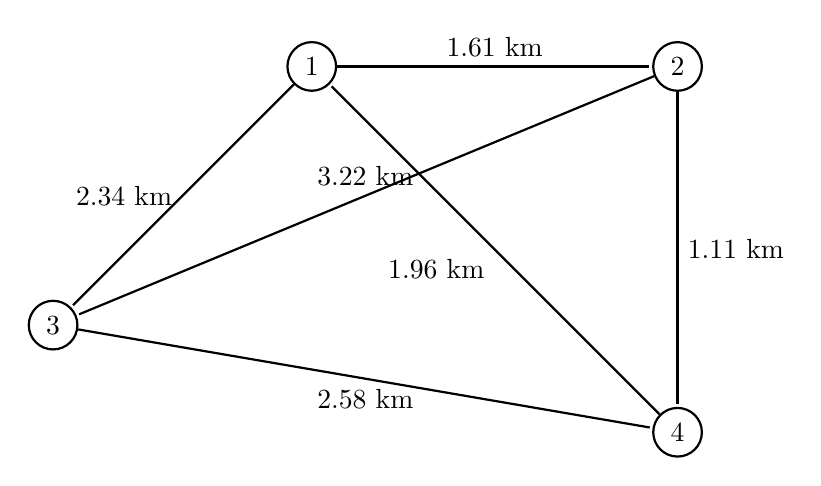
\begin{tikzpicture}[>=stealth,shorten >=1pt,auto,node distance=4cm,thick]
  \node[circle,draw] (1) {1};
  \node[circle,draw,right=of 1] (2) {2};
  \node[circle,draw,below left=of 1] (3) {3};
  \node[circle,draw,below=of 2] (4) {4};
  \path[-,draw] (1) edge node[above] {1.61 km} (2);
  \path[-,draw] (2) edge node[above] {3.22 km} (3);
  \path[-,draw] (3) edge node[below] {2.58 km} (4);
  \path[-,draw] (4) edge node[below left] {1.96 km} (1);
  \path[-,draw] (1) edge node[left] {2.34 km} (3);
  \path[-,draw] (2) edge node[right] {1.11 km} (4);
\end{tikzpicture}
\caption{A Simplified Map}
\end{figure}
\FloatBarrier % Prevent figures from floating past this point

\textbf{3.1.3. Brute Force Approach Analysis}
\begin{enumerate}
    \item Represent nodes and paths in the matrix representation (based on Figure 2)\\
    \\
    A matrix representation of a graph of 4 nodes and 6 paths:
     \[
         \bordermatrix{ & node 1 & node 2 & node 3 & node 4\cr
           node 1 & 0 & 1.61 & 2.34 & 1.96\cr
           node 2 & 1.61 & 0 & 3.22 & 1.11\cr
           node 3 & 2.34 & 3.22 & 0 & 2.58\cr
           node 4 & 1.96 & 1.11 & 2.58 & 0} \qquad
     \]

    A total of 6 permutations (branches) in a tree representation:
    \begin{figure}[h]
    \centering
    \begin{forest}
      for tree={
        circle,
        draw,
        minimum size=1.5em,
        s sep=2em,
        l sep=2em,
      }
      [1
        [2, edge label={node[midway,above left] {1.61 km}}
          [3, edge label={node[midway,above left] {3.22 km}}
            [4, edge label={node[midway,above left] {2.58 km}}
              [1, edge label={node[midway,above left] {1.96 km}}, label=below:{\footnotesize sum=9.37 km}]
            ]
            [, phantom]
          ]
          [4, edge label={node[midway,above right] {1.11 km}}
            [, phantom]
            [3, edge label={node[midway,above left] {2.58 km}}
              [1, edge label={node[midway,above left] {2.34 km}}, label=below left:{\footnotesize sum=7.64 km}]
            ]
          ]
        ]
        [3, edge label={node[midway,above right] {2.34 km}}
          [2, edge label={node[midway,above left] {3.22 km}}
            [4, edge label={node[midway,above left] {1.11 km}}
              [1, edge label={node[midway,above right] {1.96 km}}, label=below:{\footnotesize sum=8.63 km}]
            ]
            [, phantom]
          ]
          [4, edge label={node[midway,above right] {2.58 km}}
            [, phantom]
            [2, edge label={node[midway,above left] {1.11 km}}
              [1, edge label={node[midway,above left] {1.61 km}}, label=below left:{\footnotesize sum=7.64 km}]
            ]
          ]
        ]
        [4, edge label={node[midway,above right] {1.96 km}}
          [2, edge label={node[midway,above left] {1.11 km}}
            [3, edge label={node[midway,above right] {3.22 km}}
              [1, edge label={node[midway,above right] {2.34 km}}, label=below:{\footnotesize sum=8.63 km}]
            ]
            [, phantom]
          ]
          [3, edge label={node[midway,above right] {2.58 km}}
            [, phantom]
            [2, edge label={node[midway,above right] {3.22 km}}
              [1, edge label={node[midway,above right] {1.61 km}}, label=below:{\footnotesize sum=9.37 km}]
            ]
          ]
        ]
      ]
    \end{forest}
    \caption{Brute Force Algorithm Analysis for Pokémon Go Routes}
    \end{figure}
    \FloatBarrier % Prevent figures from floating past this point
    \item Calculate total distance for each permutation for every branch of the tree (as shown in Figure 3) \\
    \item Find the minimum distance (e.g. node 1 - node 2 - node 4 - node 3 - node 1 = 7.64 km)
\end{enumerate}
\FloatBarrier % Prevent figures from floating past this point
\textbf{3.1.4. Computation Costs}\\

If n presents the number of nodes, all possible permutations of node orderings is calculated as:
\[(n-1)!\]

For example, when $n = 4, 3! = 3 \times 2 \times 1 = 6$.\\

\textbf{3.1.5. Pros and Cons of Brute Force}\\

Pros
    \begin{enumerate}
        \item Simplicity: it is straightforward to implement, making them suitable for quick solutions and easy understanding.
        \item Guaranteed Solution: it guarantees finding the optimal solution, as it exhaustively explores all possibilities.
    \end{enumerate}

Cons
    \begin{enumerate}
        \item Inefficiency: it is highly inefficient, especially for large input sizes, as they examine all possible solutions without exploiting problem-specific
        \item Computational Complexity: The time and space complexity making it impractical. When $n=11$, there is $3,628,800 (10!)$ permutations.\\
    \end{enumerate}

\textbf{3.1.6. Reference}
\renewcommand{\refname}{\vspace{-2em}} % Adjust the -2em value as needed
\begin{thebibliography}{9}
\bibitem{texbook}
Joms Antony (2020), \href{https://www.youtube.com/watch?v=R_wLqwTuDzU}{Travelling Salesman Problem Intro - Brute Force Method}
\bibitem{}
Ethan Li (2024), \href{https://github.com/ethan201not404/som-discovery-topic-research-tsp/tree/main/PokemonMap}{Source code to create the Pokemon Map to demonstrate the Travelling Salesman Problem}
\end{thebibliography}


\subsection{Nearest Neighbor}     % Joshua

\textbf{3.2.1. Overview and Brief History}
\\One of the most common and intuitive solutions is known as the “Nearest neighbour” solution. Starting at an arbitrary point, lines are drawn from each successive point to the one nearest to it, hence the name “nearest neighbour”. 
\\
\\This method was specifically noted by Carl Menger, who studied the travelling salesman problem during the 1930s. The paper “\textit{On the History of Combinatorial Optimization (till 1960)”}, Karl Menger describes the difficulty of the brute-force method and also the lack of an efficient algorithm for a perfect solution, 
\\
\begin{center}
    “\textit{Of course, this problem is solvable by finitely many trials. Rules which would push the number of trials below the number of permutations of the given points, are not known.The rule that one first should go from the starting point to the closest point, then to the point closest to this, etc., in general does not yield the shortest route.}”
\end{center}\\
\textbf{3.2.2. Efficiency of Method}

\end{document}
